\documentclass{article}
\usepackage[a4paper, top=2.5cm, bottom=2.5cm, left=2.5cm, right=2.5cm]{geometry}

\usepackage[utf8]{inputenc}

\usepackage{graphicx}
\usepackage{caption}
\usepackage{subcaption}
\usepackage{float}
\usepackage{amsmath}
\usepackage{multirow}
\usepackage{algorithm}
\usepackage{algpseudocode}

\usepackage{pgfplots}
\pgfplotsset{compat=1.18}

\usepackage{hyperref}

\usepackage{xcolor}
\usepackage{minted}

\floatstyle{plain}
\restylefloat{listing}

\definecolor{codebg}{RGB}{250, 250, 250}
\definecolor{codeframe}{RGB}{200, 200, 200}

\setminted{
    style=tango,
    fontsize=\footnotesize,
    bgcolor=codebg,
    linenos=false,
    breaklines=true,
    tabsize=4,
    frame=single,
    framesep=5pt,
    rulecolor=\color{codeframe},
}

\begin{document}

\title{
  \textbf{SDC Assignment 5 - Application of EKF}
}
\author{Ying Pei Lin}
\date{Spring 2026}

\maketitle

\section{Results}

\begin{figure}[H]
    \centering
    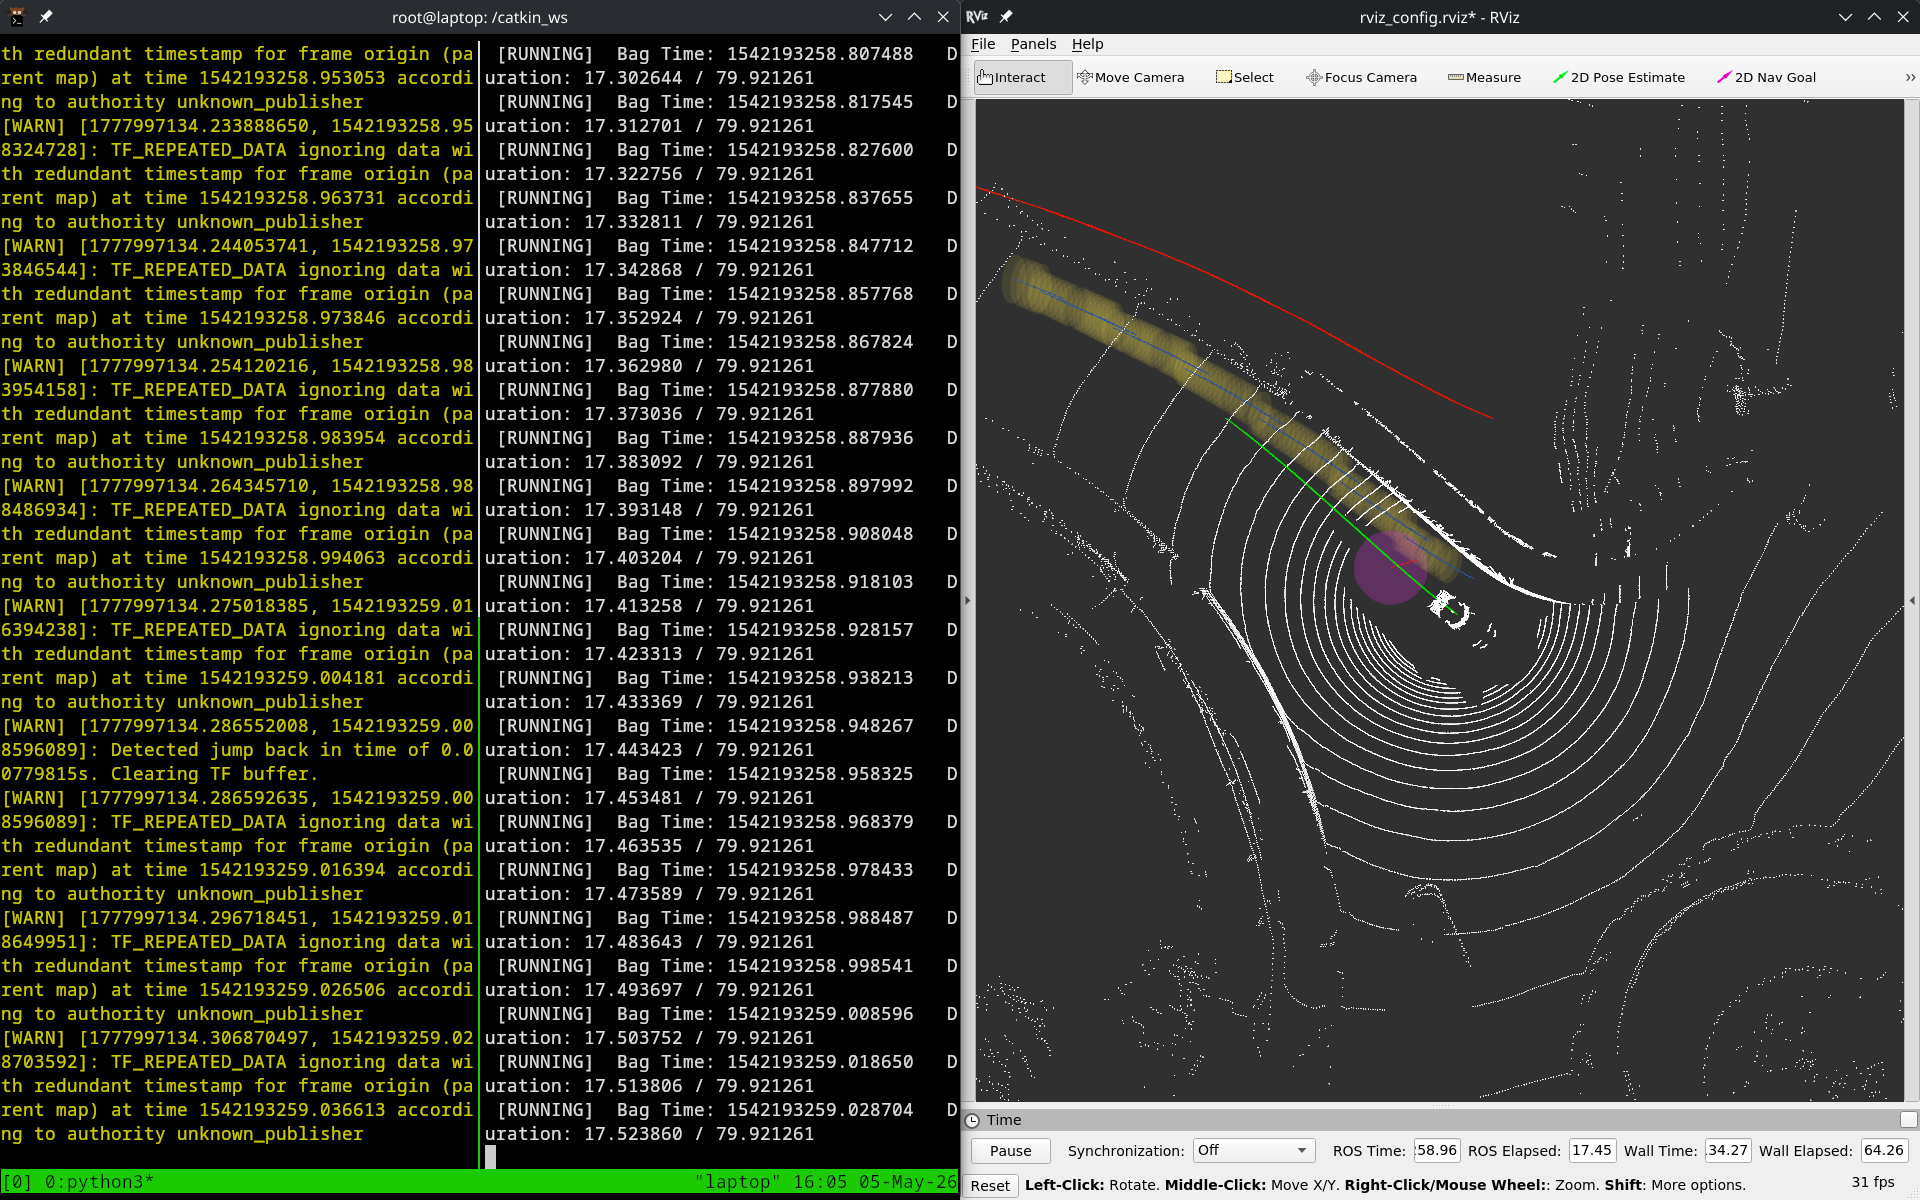
\includegraphics[width=0.8\textwidth]{running.png}
    \caption{The screenshot of the running program.}
    \label{fig:running}
\end{figure}

\textbf{YouTube Link:} \url{https://youtu.be/oK6bKV5-J7w}

\begin{figure}[H]
    \centering
    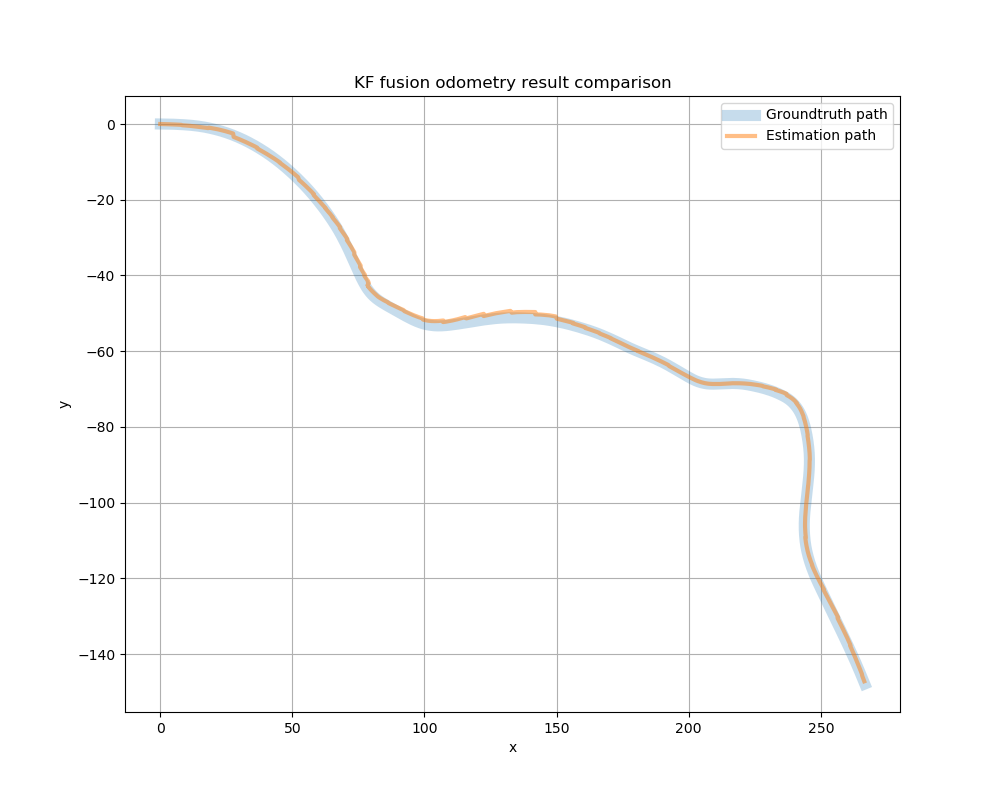
\includegraphics[width=0.8\textwidth]{result.png}
    \caption{The result of the EKF.}
    \label{fig:result}
\end{figure}

\section{Discussion}

\subsection{The design of the EKF}
The Extended Kalman Filter (EKF) is designed to estimate a 3D state vector $[x, y, yaw]^{T}$. The design consists of two main steps:

\begin{itemize}
    \item \textbf{Prediction Step (Radar Odometry):} Uses a non-linear motion model updating the pose based on local control inputs $dx$, $dy$, and $dyaw$. The state transition matrix $A$ is the Jacobian of this model. The state covariance $S$ is updated using $A$ and the process noise covariance $R$.
    \item \textbf{Update Step (GPS):} Uses an observation matrix $C$ mapping the 3D state to a 2D $[x, y]^{T}$ measurement. The Kalman Gain $K$ is computed using $C$, $S$, and the measurement noise covariance $Q$. Finally, the state and covariance $S$ are corrected based on the measurement residual.
\end{itemize}

\subsection{The covariance matrix of GPS, radar odometry}
\textbf{Definition:}
\begin{itemize}
    \item Both sensor messages provide a $6 \times 6$ covariance matrix.
    \item \textbf{Radar Odometry:} A $3 \times 3$ sub-matrix for $x$, $y$, and $yaw$ is extracted and assigned as the process noise covariance $R$.
    \item \textbf{GPS:} A $2 \times 2$ sub-matrix for $x$ and $y$ is extracted and assigned as the measurement noise covariance $Q$.
\end{itemize}

\textbf{Meaning:}
The covariance matrix represents the expected noise or uncertainty of the sensor data. A higher variance indicates lower certainty. By comparing the radar odometry covariance ($R$) and GPS covariance ($Q$), the Kalman Gain determines whether the filter should rely more on the physical motion prediction or the absolute GPS measurement.

\end{document}
